\documentclass[ngerman,hyperref={pdfpagelabels=false}]{beamer}

% -----------------------------------------------------------------------------

\graphicspath{{images/}}

% -----------------------------------------------------------------------------

\usetheme{KIT}

\setbeamercovered{transparent}
%\setbeamertemplate{enumerate items}[ball]

\newenvironment<>{KITtestblock}[2][]
{\begin{KITcolblock}<#1>{#2}{KITblack15}{KITblack50}}
{\end{KITcolblock}}

\usepackage[ngerman,english]{babel}
\usepackage[utf8]{inputenc}
\usepackage[TS1,T1]{fontenc}
\usepackage{array}
\usepackage{multicol}
\usepackage[absolute,overlay]{textpos}
\usepackage{beamerKITdefs}

\pdfpageattr {/Group << /S /Transparency /I true /CS /DeviceRGB>>}	%required to prevent color shifting withd transparent images


\title{Algorithmen 1 - Tutorium 7}
\subtitle{Sebastian Schmidt -- \textit{isibboi@gmail.com}}

\author[Sebastian Schmidt]{Sebastian Schmidt}
\institute{Arbeitsgruppe Kryptographie und Sicherheit}

\TitleImage[width=\titleimagewd,height=\titleimageht]{titel}

\KITinstitute{Arbeitsgruppe Kryptographie und Sicherheit}
\KITfaculty{Fakult\"at f\"ur Informatik}

\DeclareMathOperator{\parent}{parent}

% -----------------------------------------------------------------------------

\begin{document}
\setlength\textheight{7cm} %required for correct vertical alignment, if [t] is not used as documentclass parameter


% title frame
\begin{frame}
  \maketitle
\end{frame}

\begin{frame}{Anmerkungen zum Pseudocode}
\begin{itemize}
\item Gerne \texttt{swap} benutzen
\item Klar machen, wie Datentypen aussehen
\end{itemize}
\end{frame}

\begin{frame}{Radixsort}
\begin{itemize}
\item Ähnlich wie Bucketsort
\item Zwei Varianten: MSB (Most-Significant-Bit) und LSB (Least-Significant-Bit)
\item Beispiel: 5, 3, 4, 1, 6, 7, 2, 0
\item<2-> Warum ist Radixsort in $O(n)$?
\end{itemize}
\end{frame}

\begin{frame}{Array-Darstellung von Binärbäumen}
\begin{itemize}
\item Schreibe Knoten Ebenenweise in ein Array $A[1, \dots, n]$
\end{itemize}

\pause
Operationen:
\begin{itemize}
\item \texttt{parent(v)}
\item \texttt{leftChild(v)}
\item \texttt{rightChild(v)}
\end{itemize}
\pause
(Laufzeit?)
\end{frame}

\begin{frame}{Binäre Heaps}
\begin{itemize}
\item Heap-Eigenschaft: Bäume mit $\forall v: \parent(v) \leq v$ (MinHeap)
\end{itemize}
\end{frame}

\begin{frame}{\texttt{insert}}
Heap-Eigenschaft: Bäume mit $\forall v: \parent(v) \leq v$ (MinHeap)
\begin{itemize}
\item Hänge neues Element ans Ende
\item Stelle Heap-Eigenschaft wieder her
\end{itemize}
\pause
Laufzeit?
\end{frame}

\begin{frame}{\texttt{deleteMin}}
Heap-Eigenschaft: Bäume mit $\forall v: \parent(v) \leq v$ (MinHeap)
\begin{itemize}
\item Vertausche erstes und letztes Element
\item Entferne letztes Element
\item Stelle Heap-Eigenschaft wieder her
\end{itemize}
\pause
Laufzeit?
\end{frame}

\begin{frame}{\texttt{buildHeap}}
Heap-Eigenschaft: Bäume mit $\forall v: \parent(v) \leq v$ (MinHeap)
\begin{itemize}
\item Iteriere rückwärts über die erste Hälfte des Arrays
\item Stelle für die Nachfolger von jedem Element die Heap-Eigenschaft her
\end{itemize}
\pause
Laufzeit?
\end{frame}

\begin{frame}{Heapsort}
\begin{itemize}
\item \texttt{buildHeap} (MaxHeap)
\item \texttt{deleteMax} $\Rightarrow$ Element in die sortierte Folge einfügen
\end{itemize}
\pause
Laufzeit?
\end{frame}

\begin{frame}{Weitere Sortieralgorithmen}
\only<1>{Spaghettisort
\begin{itemize}
\item Spaghetti zuschneiden, sodass Länge den Zahlen entspricht
\item Spaghetti in die Hand nehmen und auf den Tisch stellen, sodass alle die Tischplatte berühren
\item Hand von oben auf die Spaghetti senken, bis eine berührt wird
\item Größte Spaghetti ins Array schreiben
\end{itemize}
Laufzeit?}

\only<2->{Pancakesort
\begin{itemize}
\item Pfannkuchen der Größe nach sortieren
\item Operation: Die obersten $k$ Pfannkuchen auf einmal in $O(1)$ wenden
\end{itemize}
Algorithmus?

Laufzeit?}

\only<3>{Bill Gates: $P_n < \frac{5n+5}{3}$}
\end{frame}

\begin{frame}
\centering
\vspace{-3em}
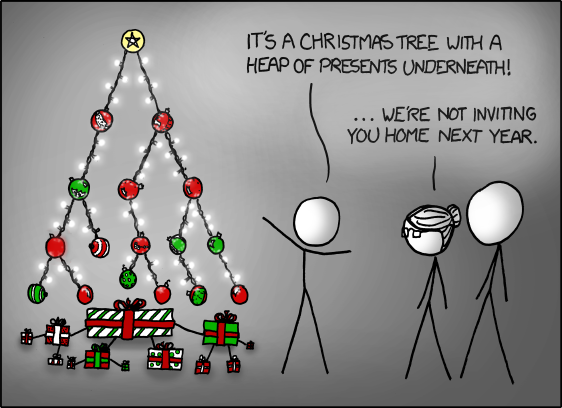
\includegraphics[width=0.95\textwidth]{tree}
\end{frame}

\end{document}
